%%%%%%%%%%%%%%%%%%%%%%%%%%%%%%%%%%%%%%%%%%%%%%%%%%%%%%%%%%%%%%%%%%%%%%%%%%%%%%%%
%                                                                              %
%            A Painless Introduction to Programming UAMMD Modules              %
%                           Chapter 3: Measuring                               %
%                                                                              %
%                          Marc Meléndez Schofield                             %
%                                                                              %
%%%%%%%%%%%%%%%%%%%%%%%%%%%%%%%%%%%%%%%%%%%%%%%%%%%%%%%%%%%%%%%%%%%%%%%%%%%%%%%%

The first two chapters have given you more than enough material to create your 
own simulations and use the output to make videos of spheres flying around and 
colliding in your own virtual world. But scientists aim at describing the real 
world, and that involves measuring interesting quantities in your system and 
relating them to material objects.

\section{Energy and linear momentum}

Physical simulations commonly measure energy. Unexpected fluctuations or drifts 
in the energy often warn us of something askew in our code. Take our bouncing 
rubber ball from the introduction. Its mechanical energy,
\begin{equation*}
  E = \frac{1}{2} m \|\mathbf{v}\|^2 + m|g|y,
\end{equation*}
should remain constant while it flies freely. The absolute value $|g|$ appears 
here instead of plain $g$ because, if you remember, we defined the acceleration 
of gravity as $g = -9.8\ \mathrm{m/s}^2$ in our code. On impact, the ball 
reduced its speed slightly, so we expect a sudden drop in $E$ every time 
the ball hits the floor. As it bounces time and again, leaking more and more 
energy, $E$ will tend towards zero.

Due to numerical rounding in the operations, we shouldn't expect a perfect 
conservation of energy but we obviously want to keep energy fluctuations low, 
below one percent, say. If you have managed to code the algorithm correctly, you 
can usually decrease energy fluctuations further by choosing smaller time steps.

Let's verify our predictions about the bouncing ball program by changing the 
output section. We'll set the mass to $100$ grams.
\begin{lstlisting}
%! codeblock: rubberBallEOutput
    if(printEverynSteps > 0
       && step % printEverynSteps == 0) {

      float m = 0.1; /* Mass */

      /* Mechanical energy */
      float E = 0.5*m*(v[0]*v[0] + v[1]*v[1]) - m*g*r[1];

      cout<<step*dt<<" "<<r[0]<<" "<<r[1]<<" "<<E<<endl;
    } //!
%! codeblockend !//
\end{lstlisting}
Note that I wrote \texttt{-m*g*r[1]} instead of \texttt{+m*g*r[1]} due to the 
negative value of \texttt{g}. Figure \ref{rubberBallE} plots the result, which 
agrees with our predictions precisely.

\begin{figure}
  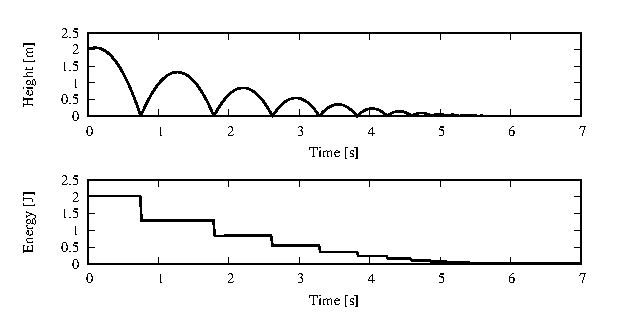
\includegraphics[width = \textwidth]{figures/rubberBallE.eps}
  \caption{\label{rubberBallE}Height (\textit{top}) and mechanical energy 
           (\textit{bottom}) of a one-hundred-gram bouncing ball versus time. 
           The energy remains constant with the ball in free flight, but a 
           fraction is lost when the ball hits the ground.}
\end{figure}

\begin{comment}
rubberBallE.cpp differs only from rubberBall.cpp in the code snippet mentioned 
above.
%! codefile: code/rubberBallE.cpp
# include <iostream>

using std::cout;
using std::endl;

int main(int argc, char * argv[])
{
  /* State of the rubber ball */
  float r[2]; /* Position (measured in metres) */
  float v[2]; /* Velocity (in metres/second) */

  float g = -9.8; /* Acceleration of gravity (in m/s^2) */

  /* Integration parameters */
  int nsteps = 10000; /* Number of time steps to calculate */
  float dt = 0.001; /* Size of time step (in seconds) */
  int printEverynSteps = 20;

  /* Initial conditions */
  r[0] = 0;
  r[1] = 2;
  v[0] = 0.5;
  v[1] = 1;

  /* Euler integration of the equations of motion */
  for(int step = 0; step <= nsteps; ++step) {
    /* New position */
    r[0] = r[0] + v[0]*dt;
    r[1] = r[1] + v[1]*dt;

    /* New velocity */
    v[1] = v[1] + g*dt;

    /* Deal with collisions */
    if(r[1] <= 0 && v[1] < 0) {
      v[0] = 0.9*v[0];
      v[1] = -0.8*v[1];
    }

    /* Output state */
    %! codeinsert: rubberBallEOutput
  }
  cout<<"# Simulated time: "<<nsteps*dt<<" seconds. #"<<endl;
  return 0;
}
%! codeend
\end{comment}

Returning to UAMMD, let's write a function that outputs the total energy of the 
system. Each interactor has a \texttt{sumEnergy} method that calculates the 
potential energy due to corresponding interaction for each particle and adds it 
to the energy vector that we access with \texttt{getEnergy}. You can add the 
kinetic energy by calling the interactor's \texttt{sumEnergy}.

To begin with, our new \texttt{getTotalEnergy} function will clear the energy 
vector and initialize the \texttt{totalEnergy} variable to zero.
\begin{lstlisting}
%! codeblock: getTotalEnergy
double getTotalEnergy(std::shared_ptr<Integrator> integrator,
                      std::shared_ptr<ParticleData> particles){
  {
    auto energy
      = particles->getEnergy(access::location::cpu,
                             access::mode::write);
    std::fill(energy.begin(), energy.end(), real(0.0));
  }

  double totalEnergy = 0; //!
  %! codeinsert: getKineticEnergy
  %! codeinsert: getPotentialEnergy
  %! codeinsert: reduceEnergyVector
%! codeblockend !//
\end{lstlisting}
Next, it sums the kinetic energies to the particle energy vector.
\begin{lstlisting}
%! codeblock: getKineticEnergy
  integrator->sumEnergy(); //!
%! codeblockend !//
\end{lstlisting}
After that, it adds in the potential energies from interactions.
\begin{lstlisting}
%! codeblock: getPotentialEnergy
  for(auto interactor: integrator->getInteractors()){
    interactor->sumEnergy();
  } //!
%! codeblockend !//
\end{lstlisting}
Finally, we accumulate all the values in the energy vector and return the grand 
total.
\begin{lstlisting}
%! codeblock: reduceEnergyVector
  {
    auto energy
      = particles->getEnergy(access::location::cpu,
                             access::mode::read);
    for(int i = 0; i < particles->getNumParticles(); ++i) {
      totalEnergy += energy[i];
    }
  }
  return totalEnergy;
} //!
%! codeblockend !//
\end{lstlisting}

Similarly, we can write a function to calculate the total linear momentum 
vector, which should remain approximately constant in the absence of external 
force fields.

\begin{lstlisting}
%! codeblock: getTotalMomentum
real3 getTotalMomentum(std::shared_ptr<ParticleData> particles){
    auto velocity
      = particles->getVel(access::location::cpu,
                          access::mode::read);
    auto mass
      = particles->getMass(access::location::cpu,
                           access::mode::read);

    real3 totalMomentum = make_real3(0.0, 0.0, 0.0);

    for(int i = 0; i < particles->getNumParticles(); ++i) {
      totalMomentum += mass[i]*velocity[i];
    }

  return totalMomentum;
} //!
%! codeblockend !//
\end{lstlisting}

We have two new tools to add to our Lennard-Jones code from chapter one. I'll 
include them above the \texttt{main} function. We'll include two novel 
parameters into the \texttt{InputParamters} data structure introduced in section 
\ref{Parameter_files}: the mass of our particles and the name of the file 
recording measured data.
\begin{lstlisting}
  real mass;
  std::string macroFile;
\end{lstlisting}
We also need the corresponding default values in the \texttt{readParameterFile} 
function,
\begin{lstlisting}
     defaultParameters<<"mass 1.0"<<endl;
     defaultParameters<<"measurementsFile LJmacro.dat"<<endl;
\end{lstlisting}
and commands to read in custom values.
\begin{lstlisting}
   parameterFile.getOption("mass",
     InputFile::Required)>>params.mass;
   parameterFile.getOption("measurementsFile",
     InputFile::Required)>>params.macroFile;
\end{lstlisting}
Within \texttt{main}, we'll set the mass of all particles to the value read in 
from \texttt{data.main}.
\begin{lstlisting}
   {
     auto mass
       = particles->getMass(access::location::cpu,
                            access::mode::write);
     std::fill(mass.begin(), mass.end(), simParams.mass);
   }
\end{lstlisting}
After we open the configuration output file, we'll also open the measurements 
file.
\begin{lstlisting}
   std::string macroFile = simParams.macroFile;
   std::ofstream macro(macroFile);
\end{lstlisting}
And within the integration loop, after printing out the configurations, we may 
write out the energy and momentum values with these lines:
\begin{lstlisting}
       macro<<step*simParams.dt<<" ";
       macro<<getTotalEnergy(integrator, particles)<<" ";
       macro<<getTotalMomentum(particles)<<" ";
       macro<<endl;
\end{lstlisting}

Table \ref{energy_conservation} displays the result of running the code with two 
different time steps, proving that a step of $dt = 10^{-3}$ in reduced units 
($\sigma = 1$, $\epsilon = 1$ and $m = 1$) should suffice for most practical 
purposes. The algorithm also achieves a reasonable conservation of the three 
components of linear momentum.

\begin{table}
    \begin{center}
			\begin{tabular}{| c | c | c |}
      \hline
			Time & \multicolumn{2}{| c |}{Total energy} \\
			$t$  &  $dt = 10^{-2}$ &  $dt = 10^{-3}$ \\
			\hline
			0    &  100000         &  100000 \\
			1    &  99988.2        &  99999.9 \\
			2    &  99987.2        &  99999.9 \\
			3    &  99988.6        &  99999.9 \\
			4    &  99987.3        &  99999.9 \\
			5    &  99986.6        &  99999.9 \\
			6    &  99985.8        &  100000 \\
			7    &  99985.4        &  100000 \\
			8    &  99985.5        &  99999.9 \\
			9    &  99985.1        &  100000 \\
			\hline
			\end{tabular}
    \end{center}
    \caption{\label{energy_conservation}Total energy of a $10^5$ Lennard-Jones 
             particles with an initial energy per particle of $\epsilon$,
             ($\sigma = 1$, $\epsilon = 1$ and $m = 1$) in a box of size $128^3$ 
             with two different time steps, $dt = 10^{-2}$ and $dt = 10^{-3}$. 
             The former gives rise to a drift that might become significant for 
             longer simulations.}
\end{table}

\section{Temperature}

The Verlet (NVE) algorithm should conserve energy and linear momentum, so we 
often rely on these quantities to signal mistakes in our code. Precisely because 
they remain constant, they do not give us much interesting information when the 
simulation runs smoothly. The values coincide approximately with those of the 
initial state we set up.

By contrast, the temperature connects the microscopic world of molecular 
collisions with the macroscopic world of flasks and thermometers. The 
equipartition theorem states that the expected value of a particle at 
equilibrium equals
\begin{equation*}
  \frac{1}{2} m \left\langle v^2 \right\rangle = \frac{3}{2}k_B T,
\end{equation*}
where $k_B$ stands for Boltzmann's constant and $T$ for the absolute 
temperature. The term on the left refers to the average kinetic energy with 
respect to the centre of mass of the system.

The equation above provides a convenient way of determining the temperature of a 
system once it equilibrates. Instead of $T$, we will write a function to 
calculate $k_BT$ and refer to this magnitude as the \textit{thermal energy}.

We start by calculating the velocity of the centre of mass, \texttt{Vcm}, and 
the total mass, \texttt{M}.
\begin{lstlisting}
%! codeblock: getThermalEnergy
double getThermalEnergy(std::shared_ptr<ParticleData> particles){
  int N = particles->getNumParticles();
  auto velocity
    = particles->getVel(access::location::cpu,
                          access::mode::read);
  auto mass
    = particles->getMass(access::location::cpu,
                           access::mode::read);

  real3 Vcm = make_real3(0.0, 0.0, 0.0);
  double M = real(0.0);

  for(int i = 0; i < N; ++i) {
    Vcm += mass[i]*velocity[i];
    M += mass[i];
  }
  Vcm /= M; //!
  %! codeinsert: getThermalKinetic
%! codeblockend !//
\end{lstlisting}
Then we calculate the total kinetic energy with respect to the centre of mass 
and return two thirds of the average kinetic energy per particle.
\begin{lstlisting}
%! codeblock: getThermalKinetic
  double kineticEnergy = real(0.0);
  for(int i = 0; i < N; ++i) {
    kineticEnergy
     += real(0.5)*mass[i]*dot(velocity[i] - Vcm, velocity[i] - Vcm);
  }

  return real(2.0/(3.0*N))*kineticEnergy;
}//!
%! codeblockend !//
\end{lstlisting}
Copying this function below \texttt{getTotalMomentum} and replacing the 
\texttt{macro<<endl;} command in the previous section with
\begin{lstlisting}
       macro<<getThermalEnergy(particles)<<endl;
\end{lstlisting}
we have written a program that can measure the equilibrium temperature of our 
system. We can now carry out our own virtual laboratory experiments. Prepare a 
simulation with some known density and internal energy, and then measure its 
temperature when it reaches equilibrium. Repeat the process changing the energy. 
The increase in internal energy, $Q$, divided by the increase in temperature, 
$\Delta T$, gives you the heat capacity $C$, because
\begin{equation*}
  C = \lim_{\Delta T \to 0} \frac{Q}{\Delta T}.
\end{equation*}
Using your simulation as a model for a substance made of neutral atoms 
(typically argon) you can make predictions of its heat capacity and compare them 
to experimental measurements.

\begin{comment}
Code blocks that we will be using below.
\begin{lstlisting}
%! codeblock: Lennard-JonesHeader
# include "uammd.cuh"
# include "utils/InputFile.h"
# include "utils/InitialConditions.cuh"
# include "Interactor/Potential/Potential.cuh"
# include "Interactor/NeighbourList/CellList.cuh"
# include "Interactor/PairForces.cuh"
# include "Integrator/VerletNVE.cuh"

using namespace uammd;
using std::make_shared;
using std::endl;
%! codeblockend

Lennard-Jones default parameters so far.
\begin{lstlisting}
%! codeblock: Lennard-JonesInputParameters
  int numberOfParticles;
  real L;
  real dt;
  real epsilon;
  real sigma;
  real mass;
  real cutOff;
  real particleEnergy;
  std::string outputFile;
  std::string macroFile;
  int numberOfSteps;
  int printEverynSteps;
%! codeblockend
\end{lstlisting}

\begin{lstlisting}
%! codeblock: Lennard-JonesReadParameterFile
  parameterFile.getOption("numberOfParticles",
    InputFile::Required)>>params.numberOfParticles;
  parameterFile.getOption("boxSize",
    InputFile::Required)>>params.L;
  parameterFile.getOption("timeStep",
    InputFile::Required)>>params.dt;
  parameterFile.getOption("epsilon",
    InputFile::Required)>>params.epsilon;
  parameterFile.getOption("sigma",
    InputFile::Required)>>params.sigma;
  parameterFile.getOption("mass",
    InputFile::Required)>>params.mass;
  parameterFile.getOption("cutOff",
    InputFile::Required)>>params.cutOff;
  parameterFile.getOption("particleEnergy",
    InputFile::Required)>>params.particleEnergy;
  parameterFile.getOption("outputFile",
    InputFile::Required)>>params.outputFile;
  parameterFile.getOption("measurementsFile",
    InputFile::Required)>>params.macroFile;
  parameterFile.getOption("numberOfSteps",
    InputFile::Required)>>params.numberOfSteps;
  parameterFile.getOption("printEverynSteps",
    InputFile::Required)>>params.printEverynSteps;
%! codeblockend
\end{lstlisting}

\begin{lstlisting}
%! codeblock: Lennard-JonesDefaultParameterList
    defaultParameters<<"numberOfParticles 100000"<<endl;
    defaultParameters<<"boxSize 128"<<endl;
    defaultParameters<<"timeStep 0.01"<<endl;
    defaultParameters<<"epsilon 1.0"<<endl;
    defaultParameters<<"sigma 1.0"<<endl;
    defaultParameters<<"mass 1.0"<<endl;
    defaultParameters<<"cutOff 2.5"<<endl;
    defaultParameters<<"particleEnergy 1.0"<<endl;
    defaultParameters<<"outputFile Lennard-Jones.dat"<<endl;
    defaultParameters<<"measurementsFile LJmacro.dat"<<endl;
    defaultParameters<<"numberOfSteps 10000"<<endl;
    defaultParameters<<"printEverynSteps 1000"<<endl;
%! codeblockend
\end{lstlisting}

\begin{lstlisting}
%! codeblock: Lennard-JonesFillMass
  {
    auto mass
      = particles->getMass(access::location::cpu,
                           access::mode::write);
    std::fill(mass.begin(), mass.end(), simParams.mass);
  }
%! codeblockend
\end{lstlisting}

\begin{lstlisting}
%! codeblock: Lennard-JonesPotential
  auto LJPotential = make_shared<Potential::LJ>(sys);
  {
    Potential::LJ::InputPairParameters LJParams;
    LJParams.epsilon = simParams.epsilon;
    LJParams.sigma = simParams.sigma;
    LJParams.cutOff = simParams.cutOff;
    LJParams.shift = true;
    LJPotential->setPotParameters(0, 0, LJParams);
  }
%! codeblockend
\end{lstlisting}

\begin{lstlisting}
%! codeblock: Lennard-JonesOutputFiles
  std::string outputFile = simParams.outputFile;
  std::ofstream out(outputFile);

  std::string macroFile = simParams.macroFile;
  std::ofstream macro(macroFile);
%! codeblockend
\end{lstlisting}

\begin{lstlisting}
%! codeblock: Lennard-JonesOutputData
    if(printEverynSteps > 0
       and step % printEverynSteps == 1) {

      auto position
        = particles->getPos(access::location::cpu,
                            access::mode::read);
      const int * index = particles->getIdOrderedIndices(access::location::cpu);

      out<<endl;
      for(int id = 0; id < numberOfParticles; ++id)
        out<<box.apply_pbc(make_real3(position[index[id]]))<<endl; //!

      macro<<step*simParams.dt<<" ";
      macro<<getTotalEnergy(integrator, particles)<<" ";
      macro<<getTotalMomentum(particles)<<" ";
      macro<<getThermalEnergy(particles)<<endl;
    }
%! codeblockend
\end{lstlisting}

Putting all the ingredients together, we get the following measurements.cu.
\begin{lstlisting}
%! codefile: code/measurements.cu

%! codeinsert: Lennard-JonesHeader

struct InputParameters {
  %! codeinsert: Lennard-JonesInputParameters
};

InputParameters readParameterFile(std::shared_ptr<System> sys)
{
  if(!std::ifstream("data.main").good()) {
    sys->log<System::WARNING>("File data.main not found. Creating file with default values.");
    std::ofstream defaultParameters("data.main");
    if(not defaultParameters.is_open()) {
      sys->log<System::CRITICAL>("Unable to create data.main file. Halting program.");
      exit(-1);
    }
    %! codeinsert: Lennard-JonesDefaultParameterList
  }
  InputFile parameterFile("data.main", sys);
  InputParameters params;

  %! codeinsert: Lennard-JonesReadParameterFile

  return params;
}

%! codeinsert: getTotalEnergy

%! codeinsert: getTotalMomentum

%! codeinsert: getThermalEnergy

int main(int argc, char *argv[]){

  auto sys = make_shared<System>(argc, argv);

  %! codeinsert: loadParameters src: chapters/first_simulation.tex

  int numberOfParticles = simParams.numberOfParticles;
  auto particles
    = make_shared<ParticleData>(numberOfParticles, sys);

  real L = simParams.L;

  %! codeinsert: LJsimulationBox src: chapters/first_simulation.tex
  {
    auto position
      = particles->getPos(access::location::cpu,
                          access::mode::write);

    auto initial =  initLattice(box.boxSize,
                                numberOfParticles, sc);

    std::copy(initial.begin(), initial.end(), position.begin());
  }

  %! codeinsert: Lennard-JonesFillMass

  using Verlet = VerletNVE;
  Verlet::Parameters VerletParams;
  VerletParams.dt = simParams.dt;
  VerletParams.initVelocities = true;
  VerletParams.energy = simParams.particleEnergy;

  %! codeinsert: Verlet src: chapters/first_simulation.tex

  %! codeinsert: Lennard-JonesPotential

  %! codeinsert: Lennard-JonesInteraction src: chapters/first_simulation.tex

  %! codeinsert: Lennard-JonesOutputFiles

  int numberOfSteps = simParams.numberOfSteps;
  int printEverynSteps = simParams.printEverynSteps;

  for(int step = 0; step < numberOfSteps; ++step) {
    integrator->forwardTime();

    %! codeinsert: Lennard-JonesOutputData
  }

  sys->finish();

  return 0;
}
%! codeend
\end{lstlisting}
\end{comment}

\section{Checkpointing}

You have spent weeks working on your code and finally managed to get it to 
perform correctly. You have set up your simulation and left it running all night 
long. In the morning, you rush to check your results and find to your dismay 
that the temperature had not yet stabilised when the program concluded. Sadly, 
you need to run it all again increasing the number of steps. Or even worse, you 
can imagine a power shortage hitting your GPU when it had been working on a 
simulation for days. I hope this conveys the importance of implementing some 
safety measures. They are well worth the effort.

You only need to save the state of the system periodically. That way, you can 
restart the run from any of these checkpoints instead of the beginning. In each 
situation, you have to decide what counts as the state of the system, that is, 
what information allows you to restore the simulation. In the case of our 
Lennard-Jones calculations, we need the values in the parameter file, the 
positions of all particles \textit{and their velocities}. But in the diatomic 
molecules simulation, you would also need the current list of bonds.

To illustrate the idea, let's include checkpointing in the Lennard-Jones system.
Among our parameters, we will have a number indicating when to back up the 
state and the name of a file from which to read it back into the program.
\begin{lstlisting}
%! codeblock: checkpointParameters
  int checkpointEverynSteps;
  std::string inputFile; //!
%! codeblockend !//
\end{lstlisting}
We can read the values in from the parameter file, but we will mark them as 
optional.
\begin{lstlisting}
%! codeblock: checkpointReadParameterFile
  params.checkpointEverynSteps = 0;
  parameterFile.getOption("checkpointEverynSteps",
    InputFile::Optional)>>params.checkpointEverynSteps;
  parameterFile.getOption("inputFile",
    InputFile::Optional)>>params.inputFile; //!
%! codeblockend !//
\end{lstlisting}
As you can see, we set the default value of \texttt{checkpointEverynSteps} to 
zero, which means no checkpointing.

When the parameters do not include an \texttt{inputFile}, the program should 
generate the initial positions and velocities.
\begin{lstlisting}
%! codeblock: checkpointInitialPositions
  if(simParams.inputFile.empty()) {
    sys->log<System::MESSAGE>("Creating new initial positions.");

    auto position
      = particles->getPos(access::location::cpu,
                          access::mode::write);

    auto initial =  initLattice(box.boxSize,
                                numberOfParticles, sc);

    std::copy(initial.begin(), initial.end(), position.begin());
  } else {
    sys->log<System::MESSAGE>("Reading initial positions and velocities from file.");
    auto position
      = particles->getPos(access::location::cpu,
                          access::mode::write);
    auto velocity
      = particles->getVel(access::location::cpu,
                          access::mode::write);

    std::string inputFile = simParams.inputFile;
    std::ifstream in(inputFile);

    for(int i = 0; i < numberOfParticles; ++i) {
      in>>position[i].x>>position[i].y>>position[i].z
        >>velocity[i].x>>velocity[i].y>>velocity[i].z;
      position[i].w = 0;
    }
  } //!
%! codeblockend !//
\end{lstlisting}

Regarding the velocities, we will set \texttt{VerletParams.initVelocities} to 
\texttt{true} only when we did not provide an \texttt{inputFile}, otherwise we 
have already read the velocities in from the file and we don't want to 
overwrite them.
\begin{lstlisting}
%! codeblock: checkpointInitVelocities
  if(simParams.inputFile.empty()) {
    sys->log<System::MESSAGE>("UAMMD will generate new velocities.");
    VerletParams.initVelocities = true;
  } else {
    VerletParams.initVelocities = false;
  } //!
%! codeblockend !//
\end{lstlisting}

Finally, after we output our data to files, we can check whether it's time to 
save the state of the system and if so copy it to a file named 
\texttt{checkpoint.}$n$\texttt{.dat} (with $n$ standing for the checkpoint 
number).
\begin{lstlisting}
%! codeblock: saveState
    if(simParams.checkpointEverynSteps > 0
       and step % simParams.checkpointEverynSteps == 1) {
      auto position
        = particles->getPos(access::location::cpu,
                            access::mode::read);
      auto velocity
        = particles->getVel(access::location::cpu,
                            access::mode::read);


      std::string checkpointFile
        = "checkpoint."
          + std::to_string(step/simParams.checkpointEverynSteps)
          + ".dat";
      std::ofstream checkpoint(checkpointFile);

      for(int i = 0; i < numberOfParticles; ++i) {
        checkpoint<<position[i].x<<" "<<position[i].y<<" "
                  <<position[i].z<<" "<<velocity[i]<<endl;
      }
    } //!
%! codeblockend !//
\end{lstlisting}

A bunch of lines such as those presented in this section might save you from 
tears many times in your career as a computational scientist.

Also, back up your data.

\begin{comment}
\begin{lstlisting}
%! codefile: code/checkpoints.cu
%! codeinsert: Lennard-JonesHeader

struct InputParameters {
  %! codeinsert: Lennard-JonesInputParameters
  %! codeinsert: checkpointParameters
};

InputParameters readParameterFile(std::shared_ptr<System> sys)
{
  if(!std::ifstream("data.main").good()) {
    sys->log<System::WARNING>("File data.main not found. Creating file with default values.");
    std::ofstream defaultParameters("data.main");
    if(not defaultParameters.is_open()) {
      sys->log<System::CRITICAL>("Unable to create data.main file. Halting program.");
      exit(-1);
    }
    %! codeinsert: Lennard-JonesDefaultParameterList
  }
  InputFile parameterFile("data.main", sys);
  InputParameters params;

  %! codeinsert: Lennard-JonesReadParameterFile
  %! codeinsert: checkpointReadParameterFile

  return params;
}

%! codeinsert: getTotalEnergy

%! codeinsert: getTotalMomentum

%! codeinsert: getThermalEnergy

int main(int argc, char *argv[]){

  auto sys = make_shared<System>(argc, argv);

  %! codeinsert: loadParameters src: chapters/first_simulation.tex

  int numberOfParticles = simParams.numberOfParticles;
  auto particles
    = make_shared<ParticleData>(numberOfParticles, sys);

  real L = simParams.L;

  %! codeinsert: LJsimulationBox src: chapters/first_simulation.tex

  %! codeinsert: checkpointInitialPositions

  %! codeinsert: Lennard-JonesFillMass

  using Verlet = VerletNVE;
  Verlet::Parameters VerletParams;
  VerletParams.dt = simParams.dt;
  %! codeinsert: checkpointInitVelocities
  VerletParams.energy = simParams.particleEnergy;

  %! codeinsert: Verlet src: chapters/first_simulation.tex

  %! codeinsert: Lennard-JonesPotential

  %! codeinsert: Lennard-JonesInteraction src: chapters/first_simulation.tex

  %! codeinsert: Lennard-JonesOutputFiles

  int numberOfSteps = simParams.numberOfSteps;
  int printEverynSteps = simParams.printEverynSteps;

  for(int step = 0; step < numberOfSteps; ++step) {
    integrator->forwardTime();

    %! codeinsert: Lennard-JonesOutputData

    %! codeinsert: saveState
  }

  sys->finish();

  return 0;
}
%! codeend
\end{lstlisting}
\end{comment}


\section{Thermostats}

Langevin thermostat

Brownian Dynamics

MSD

\section{Structure and pressure}

Post-processing

Histograms

RDF

Virial

Barostats


\begin{comment}
List of programs written in this chapter:
%! codeblock: codelist
* `rubberBallE.cpp`: A version of the `rubberBall.cpp` from the introduction
   which also outputs the mechanical energy of the ball.
* `measurements.cu`: An improvement of `superLennard-Jones.cu` that outputs the
   total energy and linear momentum, and the thermal energy (proportional to
   the absolute kinetic temperature).
* `checkpoints.cu`: An extension of `measurements.cu` with the ability restore
   simulations from saved checkpoints.
%! codeblockend
* `Langevin.cu`: Lennard-Jones molecular dynamics simulation with a Langevin
   thermostat.
* `Brownian_dynamics.cu:`: Brownian dynamics simulation with Lennard-Jones
   particles.
\end{comment}
